\chapter{Definición del problema u oportunidad} % Main chapter title
\label{sec:problema} % For referencing the chapter elsewhere, use

La evasión fiscal representa un desafío crítico para las finanzas públicas a nivel global, pero su impacto es particularmente agudo en economías emergentes y en desarrollo que enfrentan una creciente estrechez fiscal. En estos contextos, la restricción de recursos públicos amplifica el costo de oportunidad de cada peso no recaudado y exige altos estándares de eficiencia en las funciones de control del Estado.

En Chile, esta presión se ve agravada por la estructura del mercado laboral, particularmente por los altos niveles de informalidad. Según datos del Instituto Nacional de Estadísticas para el trimestre de enero a marzo de 2026 \parencite{ine2026ene}, la tasa de ocupación informal alcanzó un 26{,}5\%, lo que se traduce en más de 2{,}4 millones de trabajadores (2.498.665 personas) operando al margen del control y la protección de instituciones formales y, por ende, exentos de la retención de impuestos correspondiente. La Figura~\ref{fig:ine-informalidad} muestra la trayectoria de la tasa de ocupación informal en los últimos doce meses móviles, en los que se observa una tendencia levemente creciente (+0,7 puntos porcentuales en doce meses), con persistencia por sobre el 26\,\%.

\begin{figure}[ht]
  \centering
  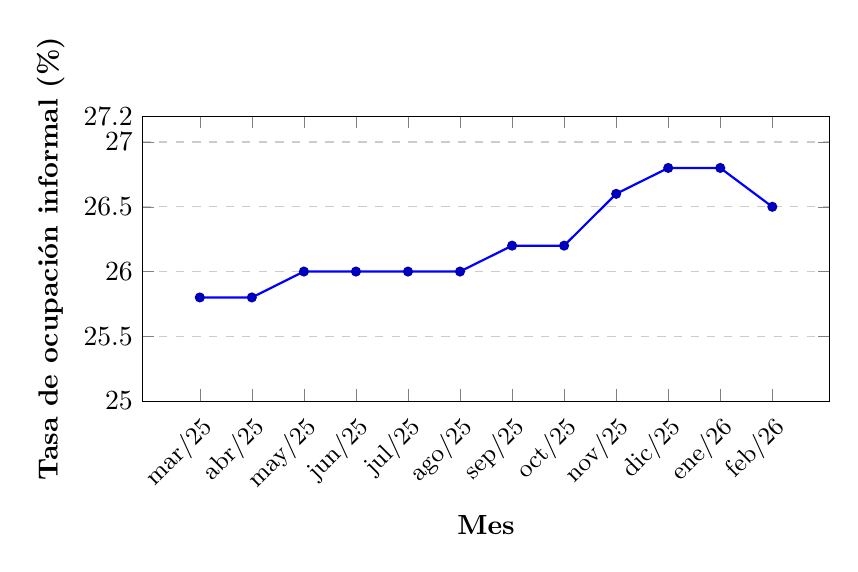
\begin{tikzpicture}
    \begin{axis}[
      width=0.85\columnwidth,
      height=5.2cm,
      xlabel={\textbf{Mes}},
      ylabel={\textbf{Tasa de ocupaci\'on informal (\%)}},
      xtick={1,2,3,4,5,6,7,8,9,10,11,12},
      xticklabels={mar/25,abr/25,may/25,jun/25,jul/25,ago/25,sep/25,oct/25,nov/25,dic/25,ene/26,feb/26},
      x tick label style={rotate=45, anchor=north east, font=\small},
      ymin=25, ymax=27.2,
      ytick={25,25.5,26,26.5,27,27.2},
      ymajorgrids=true,
      grid style={dashed,gray!40},
      mark=*,
      mark options={fill=blue!70,draw=blue!70!black,scale=0.7},
      every axis plot/.append style={thick,blue!70!black},
    ]
    \addplot coordinates {
      (1,25.8) (2,25.8) (3,26.0) (4,26.0) (5,26.0) (6,26.0)
      (7,26.2) (8,26.2) (9,26.6) (10,26.8) (11,26.8) (12,26.5)
    };
    \end{axis}
  \end{tikzpicture}
  \caption{Tasa de ocupaci\'on informal en Chile, \'ultimos doce meses m\'oviles (marzo de 2025 a febrero de 2026). \emph{Fuente}: Instituto Nacional de Estad\'isticas, Bolet\'in ENE Informalidad, edici\'on 34 \parencite{ine2026ene}.}
  \label{fig:ine-informalidad}
\end{figure}

La persistencia de la informalidad compromete directamente la sostenibilidad de los ingresos fiscales del Estado.

\section{Necesidad de optimización del proceso de auditorías}
\label{sec:optimizacion-auditoria}

Ante este escenario, el Servicio de Impuestos Internos ha transitado desde modelos de control generalistas hacia enfoques altamente focalizados. El Plan de Gestión de Cumplimiento Tributario \parencite{sii2026pgct} establece explícitamente que la estrategia de control descarta las auditorías puramente aleatorias y focaliza sus esfuerzos en contribuyentes que presentan niveles de riesgo elevados y alto impacto en la recaudación, tales como los Grupos Empresariales (que aportan el 67\,\% de la recaudación tributaria) y los Altos Patrimonios (quienes declaran cerca del 51\,\% del Impuesto Global Complementario). Este enfoque estratégico exige a la autoridad fiscal procesar continuamente historiales de comportamiento para sostener un alto impacto disuasivo y recaudatorio con el menor costo administrativo posible.

Optimizar el proceso de fiscalización implica un trade-off económico explícito. Cada auditoría ejecutada incurre en costos administrativos y de oportunidad que compiten con otras funciones del Estado, de modo que la maximización del impacto agregado no equivale a maximizar el número de fiscalizaciones sino a seleccionar contribuyentes cuya auditoría genere la mayor recaudación esperada por peso invertido. Bajo restricción presupuestaria, la autoridad fiscal necesita discriminar entre contribuyentes con alto riesgo de subdeclaración y contribuyentes de bajo riesgo, evitando la sub-fiscalización de evasores reincidentes y la sobre-fiscalización de cumplidores. Esta lógica es la que subyace al giro del SII desde controles generalistas hacia la focalización por riesgo que describe el PGCT, y es la que vuelve urgente contar con herramientas de evaluación ex-ante de las estrategias de fiscalización antes de su implementación a escala.

\section{La evasión como fenómeno social}
\label{sec:evasion-social}

La evasión fiscal no se reduce a un cálculo económico individual. La literatura ha mostrado de manera consistente que el pago de impuestos es un fenómeno intrínsecamente social, donde la moral tributaria y las decisiones de subdeclaración están fuertemente condicionadas por la interacción social y el aprendizaje comunitario \parencite{arslan2013effects, andrei2014agent}. Así, los contribuyentes no deciden en aislamiento: observan y aprenden del comportamiento y de las experiencias de fiscalización de sus pares inmediatos \parencite{arslan2013effects}, formando normas de cumplimiento que pueden ser tanto cooperativas como predatorias según la composición de su vecindad.

El fraude fiscal se propaga, por tanto, de manera horizontal a través de las redes vecinales, en lo que la literatura ha descrito como un efecto de imitación y conformidad. Investigaciones pioneras como SIMULFIS \parencite{llacer2018simulfis, noguera2014tax} demostraron que el fraude es contagioso, mientras que estudios posteriores han confirmado que la magnitud y dirección de la propagación dependen de la estructura de la red subyacente \parencite{chica2021evolutionary}. Cuando un agente observa que un vecino evadió con éxito, o que un vecino fue detectado y sancionado, ajusta su propio nivel de cumplimiento en función de esa información. Este mecanismo de propagación social implica que la evasión agregada no puede analizarse como la suma de decisiones individuales óptimas, sino como un fenómeno emergente de la interacción entre agentes heterogéneos que comparten información en una red.

\section{Modelos Basados en Agentes como herramienta}
\label{sec:abm-breve}

Para estudiar fenómenos emergentes como la evasión fiscal con componente social, los Modelos Basados en Agentes (ABM) se han consolidado como la principal herramienta metodológica en la literatura económica y computacional \parencite{hokamp2010income}. Un ABM representa a las autoridades fiscales (auditores) y a los contribuyentes como entidades autónomas y heterogéneas que interactúan en una red definida, donde cada agente actualiza su comportamiento a partir de reglas locales de aprendizaje y de la información que recibe de sus vecinos \parencite{andrei2014agent}.

El valor analítico de los ABM para el estudio de la evasión fiscal radica en que ofrecen un entorno de simulación o ``sandbox'' sin costo económico ni riesgo político, donde es posible comparar estrategias de fiscalización ex-ante, capturar propiedades emergentes que los enfoques analíticos tradicionales ignoran, y reproducir heterogeneidad tanto en los agentes como en la red social. Esta metodología es excepcionalmente útil para evaluar cómo interactúan la moral tributaria individual, el aprendizaje social entre vecinos y las decisiones del ente fiscalizador, y para examinar bajo qué condiciones cada combinación de reglas produce dinámicas de cumplimiento o evasión estables a largo plazo.

\section{Estrategias de fiscalización}
\label{sec:estrategias-fiscalizacion}

En el marco de la evaluación computacional de la fiscalización, se han propuesto tres familias principales de estrategias para la selección de contribuyentes a auditar. La primera corresponde a la \textbf{auditoría aleatoria o uniforme}, en la que cada contribuyente tiene la misma probabilidad de ser fiscalizado en cada período, independientemente de su perfil de riesgo o de su nivel de ingreso. La segunda estrategia, de \textbf{focalización por nivel de ingreso}, concentra la fiscalización en contribuyentes ubicados en tramos específicos de ingreso, bajo el supuesto implícito de que la propensión a evadir varía sistemáticamente con la renta declarada. La tercera estrategia, de \textbf{focalización estratégica o por riesgo}, prioriza a aquellos contribuyentes cuyo perfil (historial de declaraciones, ocupación, antecedentes de fiscalización) arroja un mayor puntaje de riesgo de subdeclaración, de modo que la auditoría se concentra donde la probabilidad de detección de fraude es mayor.

La literatura ha contrastado computacionalmente estas tres estrategias bajo distintas hipótesis sobre el comportamiento de los contribuyentes, encontrando que su rendimiento relativo depende de manera crítica de la velocidad del aprendizaje social en la población. En particular, el modelo de \textcite{canessa2025tax} muestra que la elección entre una estrategia de focalización estratégica y una aleatoria no es neutral: bajo condiciones de aprendizaje social lento, la auditoría aleatoria puede ser competitivamente equivalente, mientras que la focalización por nivel de ingreso tiende a subperformar de manera consistente. Estos resultados motivan un análisis cuidadoso del trade-off entre costo de fiscalización, poder disuasivo y la dinámica social subyacente.

\section{Memoria social y su degradación}
\label{sec:memoria-social}

En un ABM de cumplimiento tributario, la \textbf{memoria social} de un contribuyente corresponde a la cantidad de períodos fiscales recientes cuyos resultados de fiscalización (propios o de sus vecinos) son tenidos en cuenta al momento de actualizar su comportamiento. La intuición económica es directa: un contribuyente que recuerda haber sido auditado recientemente, o que recuerda que sus vecinos fueron sancionados, percibe un mayor riesgo de detección y eleva su nivel de cumplimiento. Por el contrario, cuando el horizonte de memoria es corto, las señales de fiscalización se diluyen rápidamente y la decisión de cada período se vuelve casi independiente de la historia reciente.

La extensión de esta memoria social es determinante para la dinámica agregada. Cuando la memoria social es corta, los agentes reaccionan primariamente a señales muy recientes y la estrategia de selección de auditoría resulta crítica para sostener la disuasión; cuando la memoria social es larga, en cambio, la información histórica se acumula en las creencias subjetivas de los agentes durante muchos períodos, lo que tiende a estabilizar las normas de cumplimiento y reduce la ventaja comparativa de las estrategias de focalización. Esta degradación natural de la relevancia temporal de la información es, a la vez, un mecanismo estabilizador de la evasión agregada y un factor que vuelve más sensible la decisión de auditoría a la elección de la estrategia. El modelo de \textcite{canessa2025tax} documenta precisamente esta interacción: bajo memoria social extendida, la focalización estratégica pierde ventaja frente a la auditoría aleatoria, mientras que la focalización por nivel de ingreso permanece consistentemente por debajo de ambas.

\section{Memoria institucional}
\label{sec:memoria-institucional}

De manera análoga, la \textbf{memoria institucional} de un ente fiscalizador corresponde a la capacidad de extender la auditoría hacia períodos fiscales anteriores al declarado. En la práctica, agencias tributarias como el Servicio de Impuestos Internos en Chile y sus contrapartes internacionales pueden revisar declaraciones de varios períodos previos al corriente, y la profundidad de esa ventana retrospectiva es una decisión de política institucional. Empíricamente, la evidencia muestra que el efecto disuasivo de una auditoría persiste en el tiempo pero se degrada a medida que la información histórica envejece, de modo que la antigüedad de los registros atenúa la probabilidad de detección efectiva de fraude pasado \parencite{debacker2018once}.

Formalmente, la memoria institucional puede caracterizarse por dos componentes: la \textbf{profundidad} (cuántos períodos hacia atrás puede revisar el fiscalizador) y un \textbf{ruido de detección} (probabilidad de que la auditoría de un período lejano identifique correctamente una subdeclaración previa, dada la degradación natural de la información). Aumentar la profundidad de revisión extiende el horizonte temporal sobre el cual el contribuyente percibe riesgo de detección, y por tanto tiende a elevar la aversión al riesgo agregada en la población; sin embargo, el ruido de detección modera este efecto, porque las auditorías sobre períodos muy antiguos tienen menor probabilidad de traducirse en una sanción efectiva. La literatura reciente no ha modelado de manera sistemática cómo interactúan esta profundidad retrospectiva del fiscalizador con la capacidad adaptativa y la memoria social de los contribuyentes, y es precisamente este vacío el que motiva la presente investigación.

\section{Problemática de la tesis}
\label{sec:problematica}

El problema que la presente tesis aborda es, por tanto, la ausencia de comprensión sistemática sobre la interacción entre la profundidad de la facultad retrospectiva del ente fiscalizador (memoria institucional con degradación de detección), la memoria social de los contribuyentes y la elección de la estrategia de fiscalización en escenarios de aprendizaje adaptativo. En particular, se desconoce bajo qué configuraciones de memoria institucional y memoria social cada estrategia de auditoría (aleatoria, por nivel de ingreso o estratégica) resulta más efectiva en términos de cumplimiento tributario y detección de fraudes a largo plazo. Responder a este problema exige formular la siguiente pregunta de investigación: ¿de qué manera la profundidad variable de la memoria institucional del ente fiscalizador (capacidad de realizar auditorías retrospectivas sujetas a ruido de detección) interactúa con la memoria social de los contribuyentes y con la estrategia de fiscalización empleada para afectar las tasas a largo plazo de cumplimiento tributario y evasión fiscal? A través de la resolución de esta interrogante, se busca entregar herramientas concretas para la calibración óptima de políticas públicas de fiscalización, identificando qué estrategia es preferible en cada contexto y maximizando el impacto de cada auditoría en ecosistemas sociales altamente adaptativos.
